\chapter{Results}
\label{ch06:results}
This chapter presents the performance results of \ac{ART} and various Kafka replication scenarios. All values in the tables are rounded to the nearest whole message, while percentages are rounded to three significant figures for consistency and accuracy. Although some scenarios involved multiple Kafka brokers, they are referred to in the singular for clarity.
% introduction to results, recap what experiments were run. percentages rounded to 3 sigfigs, everything else to nearest message.

\section{Target Adapter Performance}
\label{ch06:results:artperformance}
\ac{ART} turned out to be the slowest, on average, compared to all the Kafka scenarios measured. The average message throughput can be seen in Figure \ref{fig:chapter06:results:artavgmessage} and the specific values in Table \ref{tab:art:messagethroughput}. The message throughput lies at an average of 1.9K messages per second. The entire \ac{IS} process takes approximately 14 minutes to complete. There is some variation in the average message throughput, as seen by the standard deviation in Figure \ref{fig:chapter06:results:artavgmessage}.
% The throughput of each specific run can be found in Figure \ref{fig:appendix02:graphs:artallrunsmessage}.

\begin{table}
    \centering
    \begin{tabular}{|cc|}
        \hline
         \textbf{Average Throughput} & 1,934 msgs/sec \\
         \textbf{Median Throughput} & 1,945 msgs/sec \\
         \textbf{Maximum Throughput} & 3,136 msgs/sec \\
        \hline
    \end{tabular}
    \caption{Target Adapter Message Throughput Results}
    \label{tab:art:messagethroughput}
\end{table}

\begin{figure}[htbp]
    \centering
    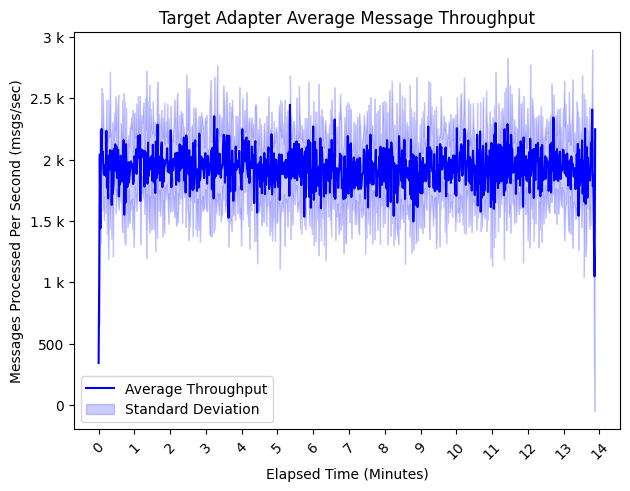
\includegraphics[width=0.75\textwidth]{chapters/images/art-performance/art-avg-message-throughput.png}
    \caption{Target Adapter average message throughput}
    \label{fig:chapter06:results:artavgmessage}
\end{figure}

The visualization of the transaction throughput can be seen in Figure \ref{fig:chapter06:results:artavgtransaction}. It was presented as a scatter plot instead of a line plot due to the throughput measurement not being continuous. \ac{ART} processed transactions in one-second bursts, with typically 1-2 second pauses in-between. This pattern is visualized in Figure \ref{fig:chapter06:results:arttransactionminute}, taken from the tracing of \ac{ART}'s processed transactions during one of the experiment runs. To take into account these processing bursts, the results in Table \ref{tab:art:transactionthroughput} include the active average throughput, which ignores the burst intervals. This allows for differentiation of how many transactions are processed on average during the bursts, as opposed to the overall average throughput.

\begin{table}
    \centering
    \begin{tabular}{|cc|}
        \hline
         \textbf{Average Throughput} & 4 transactions/sec \\
         \textbf{Active Average Throughput} & 10 transactions/sec \\
         \textbf{Median Active Throughput} & 10 transactions/sec \\
         \textbf{Maximum Active Throughput} & 12 transactions/sec \\
        \hline
    \end{tabular}
    \caption{Target Adapter Transaction Throughput Results}
    \label{tab:art:transactionthroughput}
\end{table}

\begin{figure}[htbp]
    \centering
    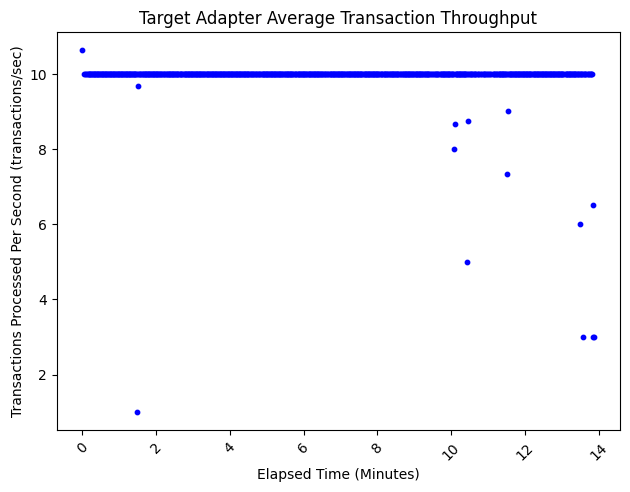
\includegraphics[width=0.75\textwidth]{chapters/images/art-performance/art-avg-transaction-throughput.png}
    \caption{Target Adapter average transaction throughput}
    \label{fig:chapter06:results:artavgtransaction}
\end{figure}

\begin{figure}[htbp]
    \centering
    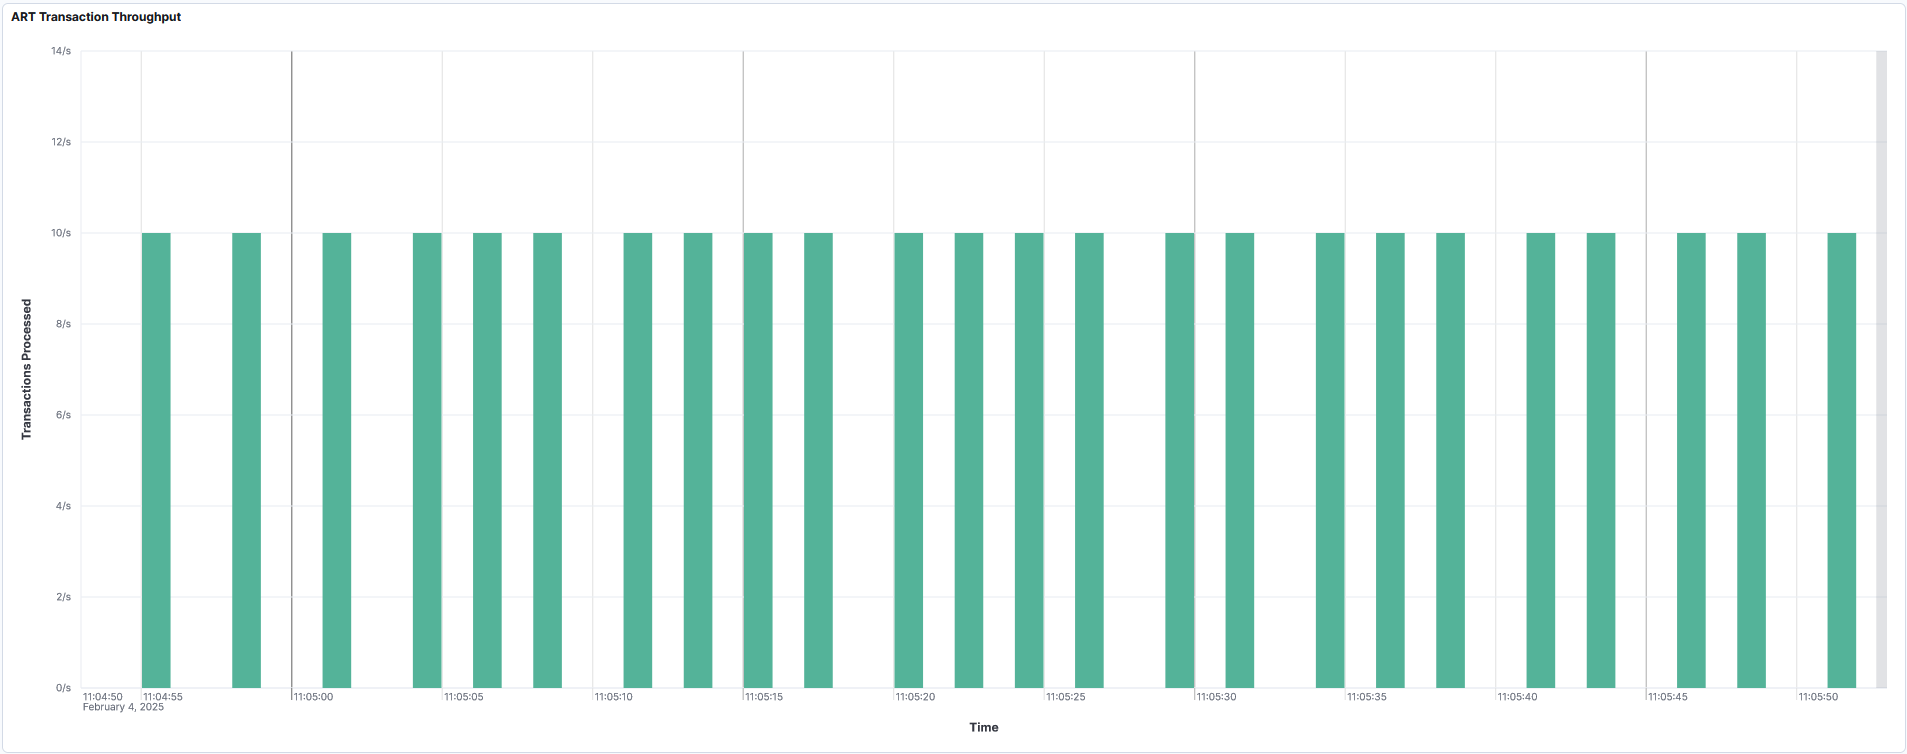
\includegraphics[width=1\textwidth]{chapters/images/art-performance/art-transaction-throughput-minute.png}
    \caption[Metric collection excerpt of Target Adapter's processed transactions]{Metric collection excerpt of Target Adapter's processed transactions (see \ref{fig:appendix02:results:arttransactionminute} for enlarged version)}
    \label{fig:chapter06:results:arttransactionminute}
\end{figure}

\section{Kafka-Based Replication Performance}
\label{ch06:results:kafakreplicationperformance}
The Kafka Connect replication solution was tested with five different configurations detailed in \ref{ch05:methodology:design:scenarios}, each representing an increasing degree of parallelization. For improved legibility, each scenario was assigned a number.

\begin{description}
    \item [Scenario 1]
    This scenario represents the "One Task, One Partition" configuration, also the one with no parallelization. The source and sink connector are running one task each. The topic is also composed of only one partition, running on a single broker.

    \item[Scenario 2]
    This scenario represents the "Three Tasks on One Worker, Three Partitions" configuration. The source and sink connector are assigned three tasks each. There are two workers, one for each connector. The topic is split into three partitions, each hosted on a broker of its own.

    \item[Scenario 3]
    This scenario represents the "Seven Tasks on One Worker, Seven Partitions" configuration, representing a higher degree of parallelization than Scenario 2. Each connector was configured to run 7 tasks, with one worker per connector. There was also an increase to 7 topic partitions, hosted on a total of 3 brokers.

    \item[Scenario 4]
    This scenario represents the "Seven Tasks on Two Workers, Seven Partitions" configuration, which has the same degree of parallelization as Scenario 3, but with task distribution on two workers per connector.
    
    \item[Scenario 5]
    This scenario represents the "20 Tasks on Five Workers, 20 Partitions" configuration and was chosen to test how well the performance scales with a significant increase in parallelization. It involves 20 tasks for the source and sink connector each. Each connector was run on five workers, and the topic was broken up into 20 partitions, with three brokers to host them.
\end{description}

In general, throughput can be seen to grow with each increase in parallelization. The message throughput, visualized for the three different pipeline components in Figure \ref{fig:chapter06:results:allscenariosmessage}, increases visibly with each scenario. The source connector in Figure \ref{fig:chapter06:results:sourceallscenariosmessage} experiences its most significant improvement in message throughput in Scenario 4, compared to Scenario 3. The same can be said for its transaction throughput, shown in Figure \ref{fig:chapter06:results:sourceallscenariostrans}. The broker's message throughput in Figure \ref{fig:chapter06:results:brokerallscenarios} experiences a similar massive increase in message throughput in Scenario 4. This was unexpected, as the significant increase in parallelization actually happened in Scenario 5 with more than double the number of tasks and workers. The rest of the scenarios were similar in pattern to the source connector. The sink connector shown in Figure \ref{fig:chapter06:results:sinkallscenarios}, on the other hand, did not show the same performance increase in Scenario 4. Instead, the performance increase occurred as expected in Scenario 5, although with very high variability and multiple drops in performance. It is interesting to note that the source connector is more performant than the sink connector in Figure \ref{fig:chapter06:results:allscenariosmessage}, with a comparatively higher message throughput observed in all scenarios.

% also talk about beggining drops in transaction throughput
% add appendix showing averages with drops more defined

The more exact measurements, with the mean, median, and maximum throughput values, can be found in Table \ref{tab:kafka:messagethroughputsource} and \ref{tab:kafka:transactionthroughput} for the source connector, Table \ref{tab:kafka:messagethroughputbroker} for the broker, and Table \ref{tab:kafka:messagethroughputsink} for the sink connector.

The average message throughput of the source connector in Table \ref{tab:kafka:messagethroughputsource} increased by 374\% in Scenario 5 compared to single-threaded Scenario 1, showcasing the extent to which parallelization impacted the connector's performance. The most significant improvement in performance, from Scenario 3 to Scenario 4, resulted in an 80.8\% increase. The increase between Scenario 4 and 5, expected to be the most significant increase in performance between scenarios due to a much higher degree of parallelization, was only improved by 16.6\%. The average source connector transaction throughput in Table \ref{tab:kafka:transactionthroughput} showed a similar pattern. There was an increase of 314\% between Scenarios 1 and 5, while the most significant improvement between the scenarios resulted in an increase of 81.5\%.

The average message throughput of the broker increased by 290\% from Scenario 1 to Scenario 5, also showing the effect of increased parallelization on performance. Similarly to the source connector, the most noticeable increase occurred from Scenario 3 to Scenario 4, measuring an improvement of 71.5\%. The performance increase between Scenario 4 and Scenario 5 was at 16\%. Generally, the broker message throughput scaled with the source connector. The broker continued to scale even in Scenarios 3, 4, and 5, where each broker hosts multiple partitions. This is visually supported when comparing Figures \ref{fig:chapter06:results:brokerallscenarios} and \ref{fig:chapter06:results:sourceallscenariosmessage}. The broker's average throughput in Table \ref{tab:kafka:messagethroughputbroker} exceeded the source connector in Scenarios 1 and 2. In Scenario 3 the broker's performance was by 2.8\% less than the source connector's, in Scenario 4 by 7.8\%, and in Scenario 5 by 8.2\%.

The sink connector's average message throughput, found in Table \ref{tab:kafka:messagethroughputsink}, diverged significantly from that of the broker and source connector. First of all, the sink connector had significantly lower overall performance. In Scenario 1, the sink connector's average message throughput is 47.9\% lower than the broker's average message throughput. The most significant increase from scenario to scenario was also different, occurring from Scenario 4 to 5 instead with an increase in 78.9\%. The total increase from Scenario 1 to Scenario 5 was by 514\%, representing by far the largest increase compared to the source connector and broker. 

Both the sink and source connectors typically experienced a noticeable variability in the average message throughput. This is especially apparent for the source connector in Figure \ref{fig:chapter06:results:sourceallscenariosmessage}, additionally more detailed in Figure \ref{fig:appendix02:results:sourcemessages}, where more prevalent performance drops occur approximately every minute of the elapsed time. The sink connector experiences similar drops in performance, as can be seen in Figure \ref{fig:chapter06:results:sinkallscenarios}, as well as in more detail in Figure \ref{fig:appendix02:results:sinkmessages}. However, the drops typically occured at different intervals than those of the source connector, and in some scenarios more often (especially in Scenario 3 and Scenario 4). The average message throughput for the broker, on the other hand, was more stable. It had no noticeable drops in any scenario, as seen in Figure \ref{fig:chapter06:results:brokerallscenarios} and in more detail in Figure \ref{fig:appendix02:results:brokermessages}.

A further observation of high variability can be seen in the greater difference between the mean and median average message throughput in each scenario in Table \ref{tab:kafka:messagethroughputsource} for the source connector and Table \ref{tab:kafka:messagethroughputsink} for the sink connector. The median in all scenarios is typically higher than the mean, indicating a possible skewed distribution of the data. A possible contribution to that could be both the low performance when just starting the \ac{IS} and the dropping performance in the very end.

% TODO: add more about sink connector and appendix ref?

\begin{figure}[htbp]
    \centering
    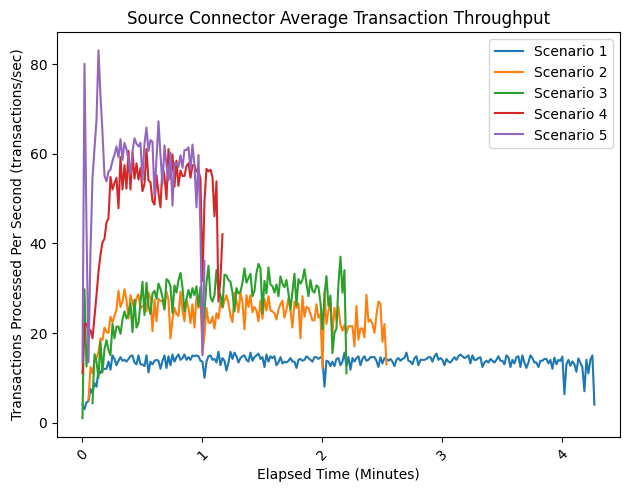
\includegraphics[width=0.75\textwidth]{chapters/images/allscenarios/source-avg-runs-all-scenarios-transaction.png}
    \caption{Source connector average transaction throughput}
    \label{fig:chapter06:results:sourceallscenariostrans}
\end{figure}

\begin{figure}[htbp]
    \centering
    \subfloat[Source connector]{\label{fig:chapter06:results:sourceallscenariosmessage}
        \centering
        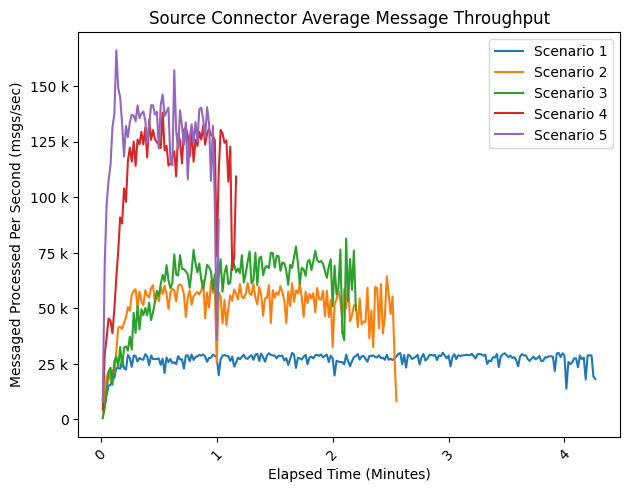
\includegraphics[width=0.75\textwidth]{chapters/images/allscenarios/source-avg-runs-all-scenarios.png}
    }
    \hfill
    \subfloat[Broker]{\label{fig:chapter06:results:brokerallscenarios}
        \centering
        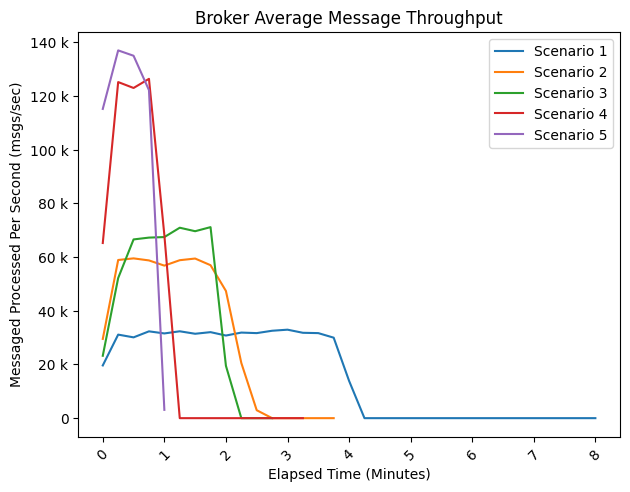
\includegraphics[width=0.75\textwidth]{chapters/images/allscenarios/broker-avg-runs-all-scenarios.png}
    }
    \hfill
    \subfloat[Sink connector]{\label{fig:chapter06:results:sinkallscenarios}
        \centering
        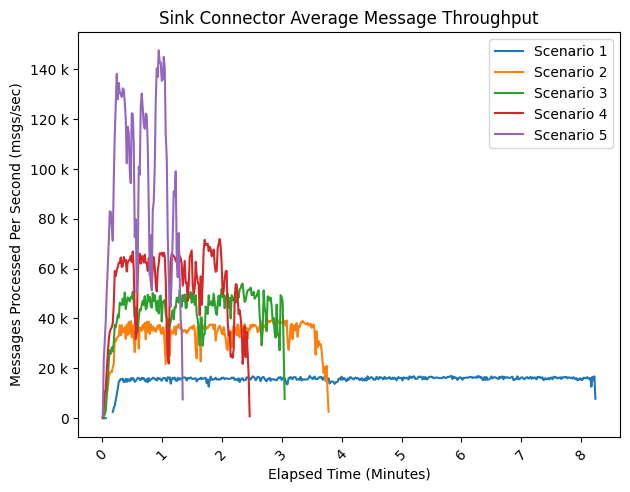
\includegraphics[width=0.75\textwidth]{chapters/images/allscenarios/sink-avg-runs-all-scenarios.png}
    }
    \hfill
    \caption{Average message throughput of various Kafka replication scenarios}
    \label{fig:chapter06:results:allscenariosmessage}
\end{figure}

\newpage
\begin{table}
    \centering
    \resizebox{\textwidth}{!}{
        \begin{tabular}{|cccccc|}
            \hline
              & \textbf{Scenario 1} & \textbf{Scenario 2} & \textbf{Scenario 3} & \textbf{Scenario 4} & \textbf{Scenario 5}\\
             \textbf{Average Throughput (msgs/sec)} & 27,090 & 50,712 & 60,952 & 110,192 & 128,496 \\
             \textbf{Median Throughput (msgs/sec)} & 28,749  & 55,827 & 64,379 & 124,469 & 134,596 \\ 
             \textbf{Maximum Throughput (msgs/sec)} & 33,968 & 71,576 & 85,824 & 147,907 & 201,680 \\
            \hline
        \end{tabular}
    }
    \caption{Kafka Replication Message Throughput Results (Source Connector)}
    \label{tab:kafka:messagethroughputsource}
\end{table}

\begin{table}
    \centering
    \resizebox{\textwidth}{!}{
        \begin{tabular}{|cccccc|}
            \hline
              & \textbf{Scenario 1} & \textbf{Scenario 2} & \textbf{Scenario 3} & \textbf{Scenario 4} & \textbf{Scenario 5}\\
             \textbf{Average Throughput (msgs/sec)} & 30,243 & 52,530 & 59,263 & 101,608 & 117,870 \\
             \textbf{Median Throughput (msgs/sec)} & 31,650 & 54,300 & 66,700 & 119,000 & 128,500 \\ 
             \textbf{Maximum Throughput (msgs/sec)} & 33,900 & 65,500 & 74,100 & 135,000 & 143,000 \\
            \hline
        \end{tabular}
    }
    \caption{Kafka Replication Message Throughput Results (Broker)}
    \label{tab:kafka:messagethroughputbroker}
\end{table}

\begin{table}
    \centering
    \resizebox{\textwidth}{!}{
        \begin{tabular}{|cccccc|}
            \hline
              & \textbf{Scenario 1} & \textbf{Scenario 2} & \textbf{Scenario 3} & \textbf{Scenario 4} & \textbf{Scenario 5}\\
             \textbf{Average Throughput (msgs/sec)} & 15,757 & 33,755 & 43,388 & 54,058 & 96,696 \\
             \textbf{Median Throughput (msgs/sec)} & 16,259 & 36,078 & 46,695 & 62,049 & 117,736 \\ 
             \textbf{Maximum Throughput (msgs/sec)} & 17,804 & 41,979 & 58,667 & 75,195 & 156,512 \\
            \hline
        \end{tabular}
    }
    \caption{Kafka Replication Message Throughput Results (Sink Connector)}
    \label{tab:kafka:messagethroughputsink}
\end{table}

\begin{table}[htbp]
    \centering
    \resizebox{\textwidth}{!}{
        \begin{tabular}{|cccccc|}
            \hline
              & \textbf{Scenario 1} & \textbf{Scenario 2} & \textbf{Scenario 3} & \textbf{Scenario 4} & \textbf{Scenario 5}\\
             \textbf{Average Throughput (transactions/sec)} & 14 & 24 & 27 & 49 & 58 \\
             \textbf{Median Throughput (transactions/sec)} & 15 & 26 & 30 & 55 & 60 \\ 
             \textbf{Maximum Throughput (transactions/sec)} & 20 & 35 & 52 & 74 & 99 \\
            \hline
        \end{tabular}
    }
    \caption{Kafka Replication Transaction Throughput Results (Source Connector)}
    \label{tab:kafka:transactionthroughput}
\end{table}
